% Created 2014-04-02 Wed 22:23
\documentclass[a4paper,12pt]{report}
\usepackage[utf8]{inputenc}
\usepackage[T1]{fontenc}
\usepackage{fixltx2e}
\usepackage{graphicx}
\usepackage{longtable}
\usepackage{float}
\usepackage{wrapfig}
\usepackage{rotating}
\usepackage[normalem]{ulem}
\usepackage{amsmath}
\usepackage{textcomp}
\usepackage{marvosym}
\usepackage{wasysym}
\usepackage{amssymb}
\usepackage{hyperref}
\tolerance=1000
\usepackage{minted}
\usepackage[bibstyle=numeric,citestyle=numeric,backend=biber]{biblatex}
\addbibresource{bibliography.bib}
\usepackage[]{hyperref}
\usepackage[]{keystroke}
\hypersetup{hidelinks}
\usepackage[]{nomencl}
\usepackage{dirtree}
\usepackage[autostyle]{csquotes}
\definecolor{dhscodebg}{rgb}{0.95,0.95,0.95}
\usepackage{menukeys}
\author{Volker Strobel}
\date{\today}
\title{My\textsc{pddl} - A Modular Knowledge Engineering System for the Planning Domain Definition Language}
\hypersetup{
  pdfkeywords={},
  pdfsubject={},
  pdfcreator={Emacs 24.3.1 (Org mode 8.2.5h)}}
\begin{document}

\maketitle
\tableofcontents

\begin{abstract}


TODO: some context

Writing and maintaining planning problems, specified in the widely
used \emph{Planning Domain Definition Language} (PDDL), can be difficult,
time-consuming and error-prone. This thesis will present myPDDL, a
toolkit that helps knowledge engineers to develop, visualize and
manipulate (\textsc{PDDL}) planning tasks. For these purposes, new,
structured PDDL projects can be created, consisting of a domain
template and associated problem files. A tool visualizes the type
hierarchy in \textsc{PDDL} domains, allowing knowledge engineers to
understand the representation structure at a glance and to keep track
of developments by a revision control. Distances between objects
specified by predicates in a problem file can be calculated with an
auxiliary tool, presenting a way of bypassing \textsc{PDDL}'s limited
modeling capacity. All these tools are based an interface that
provides a general way for reading and writing \textsc{pddl}
specifications by the use of the programming language Clojure. These
tools are made accessible in the text editor Sublime Text, where two
additional features, a syntax-highlighter and the possibility of using
code snippets for common \textsc{pddl} constructs, were implemented. A
small user study, conducted with eight inexperienced \textsc{pddl}
users, shows some initial evidence that the syntax highlighting
feature and the type diagram generator could support knowledge
engineers in the design and analysis process. So, the users detected
..\% more errors using the syntax highlighter in the same time as
non-users and the average task completion time for questions on a
hierarchical domain could be reduced by ..\%.
\end{abstract}


\chapter{Introduction}
\label{sec-1}

Have you ever struggled to devise a sequence of actions in order to
complete the Rubics' Cube? Automated planning could support you. Being
a key aspect of Artificial Intelligence (AI), AP is concerned with the
devise of a plan of actions to achieve a desired goal. It can be both
a tool for creating automated systems as well as a means for
supporting and understanding human behavior. However, the usefulness
of planning largely depends on the formalization of the underlying
problem task (source). The Planning Domain Definition Language
(\textsc{pddl}) (source) is a formal language and the quasi standard
for the description of planning tasks (source). To lay the foundations
to this thesis, a basic introduction to planning and PDDL will be
given in Chapter 2. Creating these specifications can be error-prone
and time consuming (source) \footnote{\url{http://icaps14.icaps-conference.org/workshops_tutorials/keps.html}}. Therefore, focusing on the
usability of tools for planning languages and hence facilitating the
Knowledge Engineering (KE) process is worthwhile. The aim of KE in
automated planning is thereby to turn the process of writing planning
tasks from "an art into an engineering discipline" (source). This
requires the analysis of the underlying problem itself and the
systematic use of appropriate tools specialized for developing
planning tasks.

In the scope of this thesis, the modular toolkit myPDDL (/m/odeling
/e/fficiently PDDL) was developed in order to tackle frequent needs of
knowledge engineers, like project management, efficient development,
debugging and error-detection, team collaboration features and
visualization, automation and inspecting, maintenance features
(source) and pushing the acceptance and usage of PDDL in real world
models (source). Existing tools will be critically reviewed and
compared to myPDDL in Chapter 3.

My\textsc{pddl} should support knowledge engineers in the entire
design cycle of specifying planning tasks. Therefore, it allows for
the creation of new \textsc{pddl} projects filled with templates. A
syntax highlighting feature that can allow for a faster
error-detection and help with understanding parts of \textsc{pddl}
files at a glance. As \textsc{pddl} code consists of recurrent blocks,
code snippets allow the user to insert and complete syntactic code
templates in a convenient way. Understanding the textual
representation of deep type hierarchies in domain files can be
confusing, so a further my\textsc{pddl} tool allows for the
visualization of them. \textsc{pddl}'s limited modeling possibilities
were bypassed by developing a \textsc{pddl}/Clojure interface, that
supports the conversion of \textsc{pddl} code into Clojure code and
vice versa and therefore allows, amongst others, for a partial
automation of modeling tasks. A tool based on this interface
calculates distances between objects specified in a problem file. The
modules, which are integrated in the customizable and extensible
Sublime Text editor will be described in detail in Chapter 4. Since a
main focus of the toolkit is the ease of application, a user test was
conducted (Chapter 5) with eight subjects that had no prior experience
with planning languages. The results indicate that both
error-detection and the understanding of a given domain can be
facilitated by my\textsc{pddl}. The implications, as well as general
ideas, will be discussed in Chapter 6. Finally, an outlook for future
research and developments in the field concludes this thesis (Chapter
7).
\chapter{Planning Basics and Introduction to PDDL}
\label{sec-2}

Very good for While humans\ldots{}
\url{http://citeseerx.ist.psu.edu/viewdoc/download?doi=10.1.1.362.4331&rep=rep1&type=pdf#page=7}

The human brain is an astonishing structure that allows us to get
along in a highly complex world and plan more or less rational reasons
for our past or planned actions. While computer systems are yet to
fully master these skills, the study of artificial intelligence (AI)
tries to narrow this gap. For this purpose, constructs are needed that
can represent the information about the world and the problem. The
discipline that is engaged with the integration of world information
into a computer system by a human expert is called knowledge
engineering (KE) \textcite{feigenbaum1983fifth}. In automated
planning, this is usually done using a planning language. Planning is
then the decision making process that finally leads to a sequence of
actions for solving the specified problem.

The planning domain definition language (\textsc{pddl}) is a formal
language and the quasi standard for the description of planning tasks.
\textsc{pddl} was first described in \textsc{pddl}-the planning domain
definition language (1998) and has been in constant development since
then and is currently used in version 3.1.

Consider the following (fictional) world that should be integrated
into a computer system using \textsc{}pddl:
\begin{quote}
If a hacker is hungry, he has to eat some pizza in order to exploit
vulnerable software.
\end{quote}

In this description, we can identify several constructs, that should
somehow be integrated into the computer. There are:
\begin{description}
\item[{Types of entities:}] The world consists of hackers, software and pizza.
\item[{Logical states:}] Hackers can be hungry or not, software can
\end{description}
be vulnerable or not.
\begin{description}
\item[{Actions:}] Hackers can exploit (that means hack into) software and
they can eat pizza.
\end{description}

This world description could be specified in \textsc{pddl}, using a
domain file. The domain file provides general, abstract constructs and
conditions.

Next, consider the following problem particular to this domain:
\begin{quote}
\emph{Gary} is a \emph{hungry} hacker who should
somehow exploit the vulnerable software \emph{MagicFailureApp}. Some
pepperoni pizza is laying around.
\end{quote}

Again, several constructs can be identified:
\begin{description}
\item[{Objects}] The hacker Gary, the pepperoni pizza, the software
\item[{Initial state}] Gary is hungry and the software 'MagicFailureApp'
is vulnerable
\item[{Goal state}] MagicFailureApp is exploited.
\end{description}

Assume, that Gary wants to have help of an automated planning system,
in order to plan the sequence of required actions (\emph{Who has to eat
pizza?} and \emph{What to hack?} and which one of both has to be done
first?), leading from the initial state to the goal state. These
specifications have to be formalized, this time in a problem file.
Finally, Gary will be able to fed the domain and problem file into a
planner and generate the sequence of required actions.

Summing up, \textsc{pddl} planning tasks are composed of two separate,
corresponding files:

\begin{description}
\item[{Domain file}] General, problem-independent description of types,
predicates (logical states) and actions.
\item[{Problem file}] Specification of a concrete problem within a
particular domain, expressed by the initial state
and the goal state. The values are assigned
to the templates provided by the domain file.
\end{description}


This separation allows for a powerful process of task modeling: While
general instances are described in the domain file, specific instances
of problems are created in the problem files. So, one abstract
modeling of a \emph{world} can be used for solving many problem instances.

Figure \ref{workflow} visualizes the workflow for planning in \textsc{pddl}.

TODO: Add predicates and actions to domain, 
init and goal to problem and sequence of actions to plan
\begin{figure}[htb]
\centering
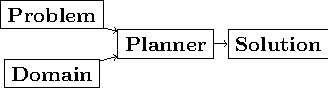
\includegraphics[width=.9\linewidth]{../img/pddl-workflow.pdf}
\caption{\label{fig:workflow}\textsc{pddl} Planning workflow}
\end{figure}
The \textsc{pddl} worklow. domain.pddl and problem.pddl represent typical
planning specification files, with the standard file extension \emph{.pddl}

\textsc{pddl} is manifold and not all parts are mandatory components
of task specifications. More complete descriptions as well as a
formulations in Backus-Naur form (BNF) can be found in
\textcite{fox2003pddl2} for \textsc{pddl} 2.2 and
\textcite{kovacs2011bnf} for \textsc{pddl} 3.1. The rest of this
section will give general design guidelines and an introduction to
\textsc{pddl}, to provide a basis for the rest of this thesis. To this
end, the syntax of common constructs of domain and problem fules shell
be investigated further in this section, in a step-by-step approach,
where both files are described by the above described example \emph{Gary's
Hacker World}.

TODO:Functions, Metrics

\section{Analysis}
\label{sec-2-1}

In order to integrate information into a computer system, first and
foremost, the problem has to be understood. How to Design Classes
(HtDC), describes a incremental process for modeling specification in
object oriented programming (\textsc{oop}). The general principles
will be transferred to \textsc{pddl}, so that in the style of the
\emph{design principles} of object oriented programming (HtDC) a stepwise,
iterative modeling process can be identified:

\begin{description}
\item[{Analysis:}] Every task specification begins by an analysis of the
informal world and the problem statement. In this design
step, one determines relevant types, adequate examples
and identifies both the initial and the goal state. One
keeps track of the analysis using any kind of list.

\item[{Type diagram:}] Based on the preceding analysis, the relationship of
the identified types is represented, using a
diagram. This can be done by pen and paper or by
means of a graph editor.
\item[{Domain definition:}] In this step, the (graphical) diagrams are
translated into \textsc{pddl}. Furthermore predicates and actions
are declared.

\item[{Problem definition:}] After completing the domain definition,
objects can be instantiated in the problem file. By means of the
predicates, declared in the domain file, the initial and goal logical
values are defined.
\end{description}

Two further steps can be identified: 

\begin{description}
\item[{Planning}] Provide domain and problem definition to a planner.
\item[{Plan analysis}] Inspect the resulting plan and optionally restart
at a earlier design step.
\end{description}

(Plan analysis can be supported by VAL or Visplan
 A further convenient method is the use of \textsc{itSimple}, so that
     the hierarchy can be translated to \textsc{pddl}.)
\section{Domain File}
\label{sec-2-2}

The domain file contains the frame for planning tasks and determines,
which types and predicates are available and which actions are possible.

\subsection{Define}
\label{sec-2-2-1}
Every domain file starts with \texttt{(define (domain DNAME) ...)} where,
\texttt{DNAME} specifies the name of the domain. It must be a string that
starts with a character, and then contains further characters(\texttt{a-z}),
numbers (\texttt{0-9}), hyphens (\texttt{-}) or underscores (\texttt{\_}). A semicolon (\texttt{;})
declares the rest of the line as comment. \textsc{PDDL}'s syntax is
case insensitive. \\
\begin{minted}[fontsize=\small,bgcolor=dhscodebg,rulecolor=\color{gray!40},frame=lines,framesep=5\fboxrule,framerule=1pt,tabsize=2]{text}
; Gary's Hacker world - A realistic example
(define (domain garys-hacker-world)
\end{minted}
\subsection{Requirements}
\label{sec-2-2-2}

\begin{itemize}
\item \textsc{pddl}: Levels of expressivity (level 1 .. 4)
\item Formal description of \textsc{pddl} tasks
\end{itemize}

\textsc{pddl} is composed of subsets of \textsc{pddl} features
\textcite[1]{mcdermott1998pddl}. As most planners only support
particular elements of \textsc{pddl}, the requirements part is useful
for a planner to determine if it is able to act on a given problem.
Often used requirements are:
\begin{description}
\item[{\texttt{:strips}}] The most elementary subset of PDDL that supports
approximately the specifications declared in the STRIPS
specification of 1971. If no requirements are
declared :strips is assumed.
\item[{\texttt{:typing}}] Enables the typification of variables (see 'Types'
below), so that variables have to be of particular type.
\item[{\texttt{:equality}}] Specifies equality (\texttt{\textbackslash{}=}) as built-in predicate, so
that
\end{description}

Besides \texttt{:typing}, Gary's hacker world will use a further requirement:

\begin{description}
\item[{\texttt{:negative-preconditions}}] Allows for the specification of
negative preconditions in actions, so that a action can only be
executed if a predicate is \emph{not} true at the beginning of the action.
\end{description}

Complete lists of requirements and their meaning can be found in
\textcite{fox2003pddl2} for \textsc{pddl} 2.1 and
\textcite{kovacs2011bnf} for \textsc{pddl} 3.1.

\begin{listing}[H]
\begin{minted}[fontsize=\small,bgcolor=dhscodebg,rulecolor=\color{gray!40},frame=lines,framesep=5\fboxrule,framerule=1pt,tabsize=2]{text}
(:requirements :typing
               :negative-preconditions)
\end{minted}
\caption{The requirements part of Gary's Hacker World}
\end{listing}
\subsection{Types}
\label{sec-2-2-3}

In the real-world, there will be often individual objects of the same
kind or \emph{type}. There may be lots of different pizza types in
existence, sharing common properties. Each pizza was made from a
similar set of ingredients and may contain similar components.

The \texttt{(:types ...)} part, \textsc{pddl} allows for declaring types and
thereby structuring the domain. Relations can be expressed by a type
hierarchy, whereby any type can be a subtype of yet another type.
Typed lists are used to assign types to variable lists. Like that,
parameters in actions can be typed, as well as arguments in
predicates, functions [extra source!]. Later, in the problem file,
objects will be assigned to types, like objects to classes in Object
Orientated Programming (OOP).

Types are declared by a list of strings, followed by a by a hypen
(\texttt{-}), followed by the the higher-level type. Every \textsc{pddl}
domain includes the built-in types \texttt{object} and \texttt{number}, whereby
every defined type is subtype of \texttt{object}.

\begin{listing}[H]
\begin{minted}[fontsize=\small,bgcolor=dhscodebg,rulecolor=\color{gray!40},frame=lines,framesep=5\fboxrule,framerule=1pt,tabsize=2]{text}
(:types hacker non-hacker - person
        white-hat gray-hat black-hat - hacker
        application system tool - software
        driver os - system
        pizza person software - object)
\end{minted}
\caption{\label{gary-types}The type hierarchy for Gary's Hacker World, consisting of different types of persons, hackers, software, The elements on the left-hand side (for example \texttt{driver os} are declared subtypes of the right-hand side (\texttt{system}). The hierarchy is expressed by using a type both on the left-hand side (for example \texttt{hacker}) and on the right-hand. \emph{Software} can be \emph{application} software, \emph{system} software or programming \emph{tools}. System software can be further divided into drivers and operating systems.}
\end{listing}

\subsection{Predicates}
\label{sec-2-2-4}
Predicates are templates for logical facts and describe the properties
of objects. They can be either true or false. The \texttt{:(predicates ...)}
part declares predicate names and number of arguments, together with
the corresponding type. The general syntax is \texttt{(p ?v1 – t1 ?v2 - t2
...)}, whereby \texttt{?} followed by a name (\texttt{v1}, \texttt{v2}), declares a
variable, and the expression (\texttt{t1}, \texttt{t2}) after the minus sign (\texttt{-})
determines the type of this variable. Thereby, the type has to be
declared in the typing section first. The number of variables
determines the arity of a predicate, ranging from zero arguments
(0-ary predicate) to any positive integer (n-ary predicate). Type
assignments for variables that have the same type and are declared
side by side can be grouped, so that \texttt{(p ?v1 ?v2 - t)} is similar to
\texttt{(p ?v1 - t ?v2 - t)}.

\begin{listing}[H]
\begin{minted}[fontsize=\small,bgcolor=dhscodebg,rulecolor=\color{gray!40},frame=lines,framesep=5\fboxrule,framerule=1pt,tabsize=2]{text}
(:predicates (has ?s - software ?p - person)
             (hungry ?p - person)
             (vulnerable ?s - software)
             (exploited ?s - software))
\end{minted}
\caption{This section declares four predicates: has (2-ary), hungry, vulnerable and exploited (1-ary).}
\end{listing}
\subsection{Actions}
\label{sec-2-2-5}

PDDL is an action-centered language. Actions are the operators in
\textsc{PDDL} and are able to change the truth value of predicates
(and therefore properties of objects), so that problems can be solved
(if there exists a solution). Actions usually consist of three parts
\begin{description}
\item[{\texttt{:parameters}}] A (typed) argument list that determines which
variables can be used in the precondition and
effect part.
\item[{\texttt{:precondition}}] Describes the applicability of an action. The
logical expression that is expressed in this part has to be
\texttt{true}, before an action can be applied.
\item[{\texttt{:effect}}] The effect describes the post-condition of an action,
that means it assigns new truth values to the mentioned
predicates.
\end{description}

\begin{minted}[fontsize=\small,bgcolor=dhscodebg,rulecolor=\color{gray!40},frame=lines,framesep=5\fboxrule,framerule=1pt,tabsize=2]{text}
;; Eat a delicious pizza
(:action eat-pizza
  :parameters (?pi - pizza ?p - person)
  :precondition (hungry ?p)
  :effect (not (hungry ?p)))

;; Exploit vulnerable software of a victim
(:action exploit        
  :parameters (?h - hacker ?s - software ?p - person)
  :precondition (and (has ?s ?p)
                     (vulnerable ?s)
                     (not (hungry ?h)))
  :effect (exploited ?s)))
\end{minted}
\section{Problem File}
\label{sec-2-3}


Planning problems are described by the pairing of domain and problem
files. Problem files declare the initial world state and the goal
state to be reached on the basis of the logical values of the
instantiated predicates. Furthermore, they create (instantiate)
concrete objects.


\subsection{Define (define (problem NAME) \ldots{})}
\label{sec-2-3-1}
Analog to the domain definition, problem files are initiated with
\texttt{(define (problem PNAME) ...)}, whereby, \texttt{PNAME} declares the name of
the problem.

\begin{listing}[H]
\begin{minted}[fontsize=\small,bgcolor=dhscodebg,rulecolor=\color{gray!40},frame=lines,framesep=5\fboxrule,framerule=1pt,tabsize=2]{text}
(define (problem garys-huge-problem)
\end{minted}
\caption{Initiating the problem file with the name garys-huge-problem}
\end{listing}
\subsection{Domain (:domain NAME)}
\label{sec-2-3-2}
Problems are designed with respect to a domain, which has to be
declared here. That means that \texttt{DNAME} in \texttt{(:domain DNAME)} and
\texttt{DNAME} \texttt{(define (domain DNAME) ...)} in the particular domain file
have to be equal.

\begin{listing}[H]
\begin{minted}[fontsize=\small,bgcolor=dhscodebg,rulecolor=\color{gray!40},frame=lines,framesep=5\fboxrule,framerule=1pt,tabsize=2]{text}
(:domain garys-hacker-world)
\end{minted}
\caption{The domain file "garys-hacker-world" is the corresponding domain file to the problem \texttt{garys-huge-problem}}
\end{listing}
\subsection{Objects (:objects \ldots{})}
\label{sec-2-3-3}
Whereby types are only templates, they can be created (instantiated)
in the =(:object\ldots{}) part. That means that types are assigned to
concrete objects.

\begin{listing}[H]
\begin{minted}[fontsize=\small,bgcolor=dhscodebg,rulecolor=\color{gray!40},frame=lines,framesep=5\fboxrule,framerule=1pt,tabsize=2]{text}
(:objects big-pepperoni-pizza - pizza
          gary - white-hat
          gisela - non-hacker 
          magicfailureapp - application)
\end{minted}
\caption{This part creates concrete objects from the type templates. So, = magicfailureapp - application= means that the object magicfailureapp is of the type application.}
\end{listing}
\subsection{Init (:init \ldots{})}
\label{sec-2-3-4}

A problem consists of two situations, the current one, which is called
the initial situation and the desired on which is called the goal state.

This part describes the initial state of the world by a list of
instantiated predicates that are declared as true. All other
predicates are assumed to be false (closed-world assumption).

\begin{listing}[H]
\begin{minted}[fontsize=\small,bgcolor=dhscodebg,rulecolor=\color{gray!40},frame=lines,framesep=5\fboxrule,framerule=1pt,tabsize=2]{text}
(:init (hungry gary)
       (vulnerable mysterious-tex-mex-mix)
       (has magicfailureapp gisela))
\end{minted}
\caption{The initial situation in Gary's Hacker World, where the hacker Gary is hungry, the application magicfailureapp is vulnerable and belongs to the non-hacker Gisela.}
\end{listing}
\subsection{Goal (:goal \ldots{})}
\label{sec-2-3-5}

The goal state refers to the situation one likes to obtain. It is
described by the logical fact that is desirable and should be reached
by the execution of the plan. In \textsc{pddl}, several goals would be
combined with =(and \ldots{}), whereby all non-specified predicates are
also nonrelevant, that means that they can be either true or false in
the goal state.

\begin{listing}[H]
\begin{minted}[fontsize=\small,bgcolor=dhscodebg,rulecolor=\color{gray!40},frame=lines,framesep=5\fboxrule,framerule=1pt,tabsize=2]{text}
(:goal (exploited magicfailureapp)
\end{minted}
\caption{In the end, the software magicfailureapp should be exploited.}
\end{listing}
\section{Planning}
\label{sec-2-4}

The effort of the formalization of the planning task will be finally
rewarded by the automatic generation of the plan.

The input to the planning software is a domain file and a
corresponding problem file, the output is a sequence of actions (the
\emph{plan}), leading from the initial state to the goal state.

Due to the yearly \textsc{icaps}, there is a broad range of available
planners. This thesis uses the planner SGPlan\(_{\text{6}}\)
\textcite{hsu2008sgplan}, a 'extensive' (in the sense of its
supporting features) planner for both temporal and non-temporal
planning problems.


An overview of different planners is given at
\url{http://ipc.informatik.uni-freiburg.de/Planners}.

Additionally, the quality of error messages is very diversified. While
some simple state: error occured, other list the problem and the line.

\chapter{Related Work}
\label{sec-3}


\section{PDDL Studio}
\label{sec-3-1}
\textsc{pddl} Studio \parencite{plch2012inspect}, is an application
for creating and managing \textsc{pddl} projects. A project is
regarded as a collection of \textsc{pddl} files. Its IDE is inspired
by Microsoft Visual Studio and imperative programming paradigms. Its
core function is the \textsc{pddl} project management, consisting of
managing \textsc{pddl} projects and creating, adding , so that
corresponding as well as inspecting, analyzing and modifying the
underlying domain and problem files. Besides general editing features
like line counting, bracket matching and auto-save, it supports
\textsc{pddl} specific editing features including syntax highlighting,
code folding (collapse code blocks to see only a single visible line)
and context aware code completions, all based on a \textsc{pddl} to
\textsc{xml} parser. This parser can also be used to convert
\textsc{pddl} to \textsc{xml} files and vice versa for domain and
problem file editing. Also based on this parser is a included,
sophisticated on the fly error detection, recognizing both syntax
errors (missing keywords, parentheses, etc.) and semantic errors
(wrong type of predicate parameters, misspelled predicates, etc.). As
semantic errors can be of a \emph{interfile nature}, meaning that there is
a mismatch between domain and problem file, \textsc{pddl} Studio can
detect such errors. TODO: Explain further. The code completion feature
allows for the selection of completion suggestions for a for standard
\textsc{pddl} constructs and dynamic list completions, that were used
in the current project (TODO: technical terms!). An interface allows
the integration of command line planners in order to run and compare
different planning software. that means syntax and semantic checking,
syntax highlighting, code completion and project management. While
colors for highlighted code can be customized, the background color of
the tool is always white. In its most recent version (of 15.6.2012),
\textsc{pddl} Studio's parser supports \textsc{pddl} 1.2, the official
language of the first and second IPC in 1998 and 2000 respectively.
Since then, \textsc{pddl} has largely evolved, the most recent and
most powerful version is \textsc{pddl} 3.1, supporting amongst others
durative actions. \textsc{pddl} Studio does not support the insertion
of larger code skeletons (called \emph{snippets} in this thesis). The
customization features (without editing the C source code) are limited
to the choice of font style and color of highlighted \textsc{pddl}
expressions. \textsc{pddl} Studio is written as standalone program,
meaning that there are no \textsc{pddl} independent no extensions .
\section{ItSIMPLE}
\label{sec-3-2}
The \textsc{itSimple} project is a graphical interface that allows for
designing planning models in an object-oriented approach, using Unified
Modeling Language (UML) diagrams. UML was invented in order to
standardize modeling in software engineering (SE). It consists of
several part notations, the here presented tool uses the 'class
diagram' notation, as \textsc{pddl} types and classes in OOP have strong
resemblance (see Tiago 2006, p 535). \textsc{itSimple} proposes UML.P (UML in a
Planning Approach), a UML variant that specifies a structure for Class
(domain specification), Object (problem specification) and StateChart
Diagrams (dynamic behavior of actions).

\textsc{itSimple}'s main focus is to support knowledge engineers in the initial
stages of the design phase by providing an opportunity for the
transition of the informality of real world requirements to domain
models as formal specifications. The assertive statement is to provide
a tool for a \enquote\{disciplined process of elicitation, organization
and analysis of requirements\}. Petri Nets can be generated from the
UML model and be used to validate the planning domain's static and
dynamic bevahior. Finally, a \textsc{pddl} representation can be generated from
the UML diagram, if required, edited, and finally used as input to a
variety of planning systems. The generated plan can be inspected using
the in-build plan analysis, consisting of a plan visualization and
plan simulation (TODO: write some more info). \textsc{itSimple}'s mdoeling
workflow is unidirectional, as changes in the \textsc{pddl} domain do not
affect the UML model and UML models have to be modeled manually,
meaning that they cannot by generated using \textsc{pddl}.

Starting in version 4.0 (currently in beta status as of writing of
this thesis) \textsc{itSimple} expanded its features to allow the creation of
\textsc{pddl} projects from scratch (i.e. without UML to \textsc{pddl} translation
process). Thus far, the \textsc{pddl} editing features are basic (see YouTube
video). A minimal syntax highlighting feature recognizes \textsc{pddl} keywords
and variables. Furthermore, \textsc{itSimple} provides templates for \textsc{pddl}
constructs (similar to the code snippets presented in this thesis),
consisting of requirement specifications, predicates, actions, goals
and initial definitions. 

\textsc{itSimple}'s original and main design approach is reversed to the
process presented in this paper. While \textsc{itSimple} generates \textsc{pddl} models
from UML specifications, my\textsc{pddl} generates type diagrams from \textsc{pddl}. So,
while \textsc{itSimple} focuses on the initial design phase, the tools
presented here are made for later stages.


Agent, environment, problems of semantic assumptions, disadvantages,
advantages, associations (many arrows could be distracting),

\emph{my\textsc{pddl}} allows for a representation of a arbitrary, n-ary predicates,
without making assumptions about semantics. On the one hand this
allows for a visualization of any \textsc{pddl} domain (and n-ary predicates),
while one the other hand (that means, if semantic assumptions are made
correctly, U

\textsc{itSimple}'s modeling process is focused on a graphical design process
and the newly added \textsc{pddl} editing features are basic, consisting of
highlighted keywords and variables. The templates primarily insert
\textsc{pddl} keywords, without showing the required syntax (e.g. \texttt{(:predicates
...)} instead of \texttt{(:predicates (predicate-name ?x - object)}. \textsc{itSimple}
is not customizable (without editing the Java source code). It is not
possible to define custom key shortcuts for commands. General editor
features, like to displaying line numbers, matching brackets or code
folding are not (yet) supported.

\emph{my\textsc{pddl}} shell support both, the initial design process of creating
domains (by code snippets and the Clojure interface) and the later
step of checking validity of existing domains and problems by the
type generator (and possibly extending them).
\section{PDDL-Mode for Emacs}
\label{sec-3-3}
\textsc{pddl}-mode (announced 2005 in a mailing list) is a major Emacs
mode for browsing and editing \textsc{pddl} 2.2 files. It provides
syntax highlighting by basic pattern matching of \textsc\{pddl]
keywords, variables and comments, regardless of the current context.
Furthermore, its provides automatic indentation and completions and
bracket matching. Code snippets for the insertion of domains, problems
and actions are provided. A declaration entry in the Emacs menu bar
shows all actions  in the current \textsc{pddl} file and
allows for jumping to the definition.

Being an Emacs mode, \textsc{pddl}-mode is highly and easily customizable. Text
editor features, like auto-completion, can be extended independently
of this mode, by installing further Emacs modes.

\emph{my\textsc{pddl}} uses Sublime Text, an editor, that is an extensible
and customizable editor as well. The syntax highlighting feature of
\emph{my\textsc{pddl}} supports all \textsc{pddl} versions, up to the most
recent version 3.1. in contrast to \emph{\textsc{pddl}-mode},
\emph{my\textsc{pddl}-h's} syntax highlighting feature is context-dependent
and more extensive, as it can recognize almost any \textsc{pddl}
construct and highlight it according to its semantic.

By syntax highlighting, both tools can support code navigation,
however, \emph{\textsc{pddl}-mode} does not allow for an fast and evident error
detection.
\section{Conclusion \& Summary}
\label{sec-3-4}
As it can be seen, there is need for an up-to-date, customizable, text
editor with \textsc{pddl} support, that supports the current standard
\textsc{pddl} 3.1. myPDDL integrates and expands features described in
this section, while keeping an focus on application, efficiency and
customization opportunities. 
\chapter{Software Engineering Tools for AI Planning}
\label{sec-4}

\section{Statement of Problem}
\label{sec-4-1}

Writing and maintaining \textsc{pddl} files can be time-consuming and
cumbersome \textcite{li2012translating}. To this end, a collection of
extensible development tools (\emph{my\textsc{pddl}}) shell support and
facilitate the \textsc{pddl} task design process and reduce potential modeling
errors. Main goals are a fast and reliable (or good) design process
that should support the collaboration between knowledge engineers and
thereby promote the use of \textsc{pddl} in real-world applications.

\emph{my\textsc{pddl}} is a extensible, modular system, designed for
supporting knowledge engineers in the process of writing, analyzing
and expanding \textsc{pddl} domains and problems. Based on a general
interface between \textsc{pddl} and Clojure, allowing for file input
(reading \textsc{pddl}) and output (\textsc{pddl} domain and problem
generation), the following integral parts of \emph{my\textsc{pddl}} will be
presented in the following sections:

\begin{description}
\item[{my\textsc{pddl}-new}] Create a new \textsc{pddl} project folder with domain and
problem skeletons
\item[{my\textsc{pddl}-gen}] A \textsc{pddl} type diagram generator for analyzing the
structure of type and object hierarchies.
\item[{my\textsc{pddl}-loc}] Automated distance calculation for \textsc{pddl} locations
\item[{my\textsc{pddl}-syn}] A syntax highlighting feature that colorizes
\textsc{pddl} constructs by its context
\item[{my\textsc{pddl}-snp}] Code snippets (templates), which can be inserted in
\textsc{pddl} files.
\item[{my\textsc{pddl}-sub}] The integration of \emph{my\textsc{pddl}-syn}, \emph{-snip} and \emph{-gen}
                into a environment to be used in Sublime Text
\end{description}

myPDDL is focused on customizability and extensibility, ranging from
the choice of key bindings and themes to the adaptability of the code
snippets to the point of adding a new module based on the general
interface.

TODO: Mindmap for modular hierarchy.
\section{General Interface between \textsc{pddl} and Clojure (/my\textsc{pddl}-i/f)}
\label{sec-4-2}

Being a planning language, \textsc{pddl}'s modeling capabilities are
limited. For this reason, a interface with a programming seems
reasonable and can partly automate the modeling process as well as
reduce the modeling time (see e.g. distance calculator). Furthermore,
In IPC, task generators are used to write extensive domain and problem
files. As \textsc{pddl} is used to create more and more complex
domains (SOURCE1, SOURCE2, SOURCE3, \ldots{}).

In this section, a general approach for generating \textsc{pddl} constructs,
but also for reading in domain and problem files, handling, using and
modifying the input, and generating \textsc{pddl} files as output, will be
presented.


While it seems to be reasonable to further extend \textsc{pddl}'s modeling
capability to at planning time instead of modeling time, a modeling
support tool as preprocessor is appropriate in any case
(\url{http://orff.uc3m.es/bitstream/handle/10016/14914/proceedings-WS-IPC2012.pdf?sequence=1#page=47})

As \textsc{pddl}'s syntax is inspired by \textsc{lisp} \parencite[64]{fox2003pddl2},
using a \textsc{lisp} dialect for the interface seems reasonable, as file input
and output methods can use s-expressions instead of regular
expressions. This way, \textsc{pddl} expressions can be extracted from a task
specification and written back in a similar manner, and parts of \textsc{pddl}
files can be accessed in a convenient way. This thesis uses Clojure
\parencite{hickey2008clojure}, a modern \textsc{lisp} dialect that runs on the
Java Virtual Machine.

The interface is built on two methods:
\begin{description}
\item[{read-construct(keyword,file)}] Allows for the
extraction of a \textsc{pddl} construct, specified by its name.
\item[{add-construct(file,position,part)}] Provides a means for adding
\textsc{pddl} constructs to a specified position, indicated by a
keyword.
\end{description}

Once a part is extracted and represented in Clojure, the processing
possibilities are manifold. An implementation using the
\texttt{read-construct} method is myPDDL-gen. The combination of these two
methods allows for the manipulation of existing \textsc{pddl} files,
as well as the creation of new files, as shown by myPDDL-loc. Possible
further applications could consist of domain and problem generators, \ldots{}
\section{Create PDDL Projects (myPDDL-new) p}
\label{sec-4-3}
Prior to each implementation of a \textsc{pddl} task specification
stands the creation of at least one domain and a belonging problem
file. In order to facilitate the creation of these files and to keep
track of their development, \emph{my\textsc{pddl}-new} creates a structured
\textsc{pddl} project folder, given a project name (Figure
\ref{fig:mypddl-new-project-folder}).

\begin{figure}[] 
  \dirtree{%
  .1 project-name.
  .2 dot.
  .2 diagrams.
  .2 domains.
  .2 problems.
  .2 solutions.
  .2 domain.pddl.
  .2 p01.pddl.
  .2 README.md.
  }
\caption[]{\label{fig:mypddl-new-project-folder}The project folder structure created by myPDDL-new. project-name is chosen by the user.}
\end{figure}

In this project folder, the domain file \texttt{domain.pddl} and the problem
file \texttt{p01.pddl} (in folder \texttt{problems}) are filled with basic
\textsc{pddl} skeletons (TODO: remove this sentence or add
functionality or even better: specify a template, which can be
added!).\\
The \texttt{domains}, \texttt{dot} and \texttt{diagrams} folders are created for the use
with \emph{my\textsc{pddl}-gen}, which will save its generated output to
these folders and thereby allows for a basic version control system
(see section 123). \\
As domain files usually have multiple problem files, the \texttt{problems}
folder is designed for the collection of all associated problem files.
$\backslash$\Recognizing, that most knowledge engineers do not write any
documentation related to the specified planning task (source: Shah,
Chrpa), \texttt{README.md} is a Markdown file, which is, amongst others,
intended for information about the author(s) of the project, contact
information, informal domain and problem specifications, TODOs and
licensing information.

The functionality of \emph{my\textsc{pddl}-new} is available trough a
command line interface, which allow for an integration of ST (and
every other tool that holds an interface for command line). New
\textsc{pddl} projects can be generated by invoking the following
command:

\begin{minted}[fontsize=\small,bgcolor=dhscodebg,rulecolor=\color{gray!40},frame=lines,framesep=5\fboxrule,framerule=1pt,tabsize=2]{bash}
$ java -jar path/to/my\textsc{pddl}.jar new NAME
\end{minted}

This approach should support an structured and organized design
process. The choice of a folder structure (instead of a project file)
has the advantage of being readable and customizable by every editor.
So the need for team work (source, shah KE) is tackled by using a
structures project folder where and changes can be seen in the view of
the diagram. + Git connection
This directory organization is intended to contain a single or just a
few domain files in one project, stored in the project root directory,
while problem files are stores in the subfolder problems.
\section{Syntax Highlighting}
\label{sec-4-4}

\textbf{*} Statement of Problem
\label{sec:syntax}


Writing extensive domain and problem files is a cumbersome and
time-consuming task \textcite{zhuo2010learning}. Addtionally, longer
files can get quickly confusing. Therefore, it is convenient to have a
tool that supports editing these files. Syntax highlighting, a common
feature of text and code editors, describes the feature of displaying
code in different styles (colors, fonts) according to the category of
terms. In order to facilitate editing PDDL files, a syntax
highlighting plug-in for the text and source code editor Sublime Text
\cite{sublimetext2,sublimetext3} is proposed.

The process of writing \textsc{pddl} files usually involves extending
them and making continual amendments to them. SH provides code in a
more readable way and can help to find and fix code errors quickly
(see evaluation). 


\subsection{Implementation and Customization}
\label{sec-4-4-1}
ST syntax definitions are written in property lists in the \textsc{xml} format.

For the ease of creation, the \textsc{pddl} syntax highlighter is
implemented by the use of the ST plug-in \textcite{aaapackagedev}. So,
the definitions can be written in YAML in converted to Plist
\textsc{xml} later on. \textcite{aaapackagedev} is a ST plugin, that
helps to create, amongst others, ST packages, syntax definitions and
'snippets' (re-usable code).

By means of Oniguruma regular expressions \parencite{kosako}, scopes
are defined, that determine the meaning of the \textsc{pddl} code
block. ST themes highlight different parts of the code by the use of
scopes. Scopes are defined by the use of regular expressions (regexes)
in a tm-Language file. The scope naming conventions mentioned in the
\citetitle{textmate} are applied here. By the means of the name, the
colors are assigned according to the current used ST theme. That means
that colors are not assigned per se, but dependently on the current
scheme. Through that, experienced users can use their default theme
and all can easily change the colors by changing the scheme. Different
ST themes display different colors (not all themes support all naming
conventions).

The syntax highlighting is intended for \textsc{pddl} 3.1, but is
backward compatible to previous version. It's based on the Backus-Naur
Form (BNF) descriptions, formulated in
\textcite{kovacs2011bnf,fox2003pddl2,mcdermott1998pddl}.

The pattern matching heuristic that is implemented by the use of
regular expressions is used for assigning scopes to the parts of the
file. As a result of \textsc{pddl}'s \textsc{lisp}-derived syntax,
\textsc{pddl} uses the s-expression format for representing
information (SOURCE!). So, the semantic of a larger \textsc{pddl} part
(sexpr) can be recognized by a opening parenthesis, followed by
\textsc{pddl} keyword and finally matched closing parentheses
(potentially containing further sexpr). These scopes allow for a
fragmentation of the \textsc{pddl} files, so that constructs are only
highlighted, if they appear in the right section.

The YAML-tmlanguage file is organized into repositories, so that
expressions can be re-used in different scopes. This organization also
allows for a customization of the syntax highlighter. The default 

The first part of the \textsc{pddl}.YAML-tmlanguage
describes the parts of the \textsc{pddl} task that should be highlighted. By
removing (or commenting) include statements, the syntax highlighter is
adjustable the user's need.


\begin{figure}[htb]
\centering
\includegraphics[width=.9\linewidth]{/home/pold/Documents/BA/org-ba/thesis/img/coffee_errors_img.png}
\caption{\label{Screenshot-in-Sublime-Text-3}Coffee domain with and without syntax highlighting}
\end{figure}
\url{file:///home/pold/Documents/BA/org-ba/thesis/img/coffee_errors_no.pngp}

\subsection{Usage and Customization}
\label{sec-4-4-2}

\textsc{myPddl} can be installed via Package Control or by placing the
files of this repository (\ldots{}) have to be placed in the ST packages folder
(\url{http://www.sublimetext.com/docs/3/packages.html}). Following, the
features can be activated by changing ST's syntax to \textsc{pddl}
(\texttt{View->Syntax->\textbackslash{}textsc\{pddl\}}).


By using ST as editor, language independent ST features are supported,
like auto completion of words already used in this file, code folding
and column selection, described in the Sublime Text 2 Documentation.

The \textsc{pddl}.YAML-tmlanguage file is split in two parts:

By default, all scopes are included.


\begin{enumerate}
\item Workflow
\label{sec-4-4-2-1}
Gary creates a new \textsc{pddl} project using the command line, to this end he
types

\begin{minted}[fontsize=\small,bgcolor=dhscodebg,rulecolor=\color{gray!40},frame=lines,framesep=5\fboxrule,framerule=1pt,tabsize=2]{bash}
$ java -jar pddl.jar new hacker-world
\end{minted}

changes into that directory 

\begin{minted}[fontsize=\small,bgcolor=dhscodebg,rulecolor=\color{gray!40},frame=lines,framesep=5\fboxrule,framerule=1pt,tabsize=2]{bash}
$ cd bulb-world
\end{minted}
and renames the file domain.pddl to 

\begin{minted}[fontsize=\small,bgcolor=dhscodebg,rulecolor=\color{gray!40},frame=lines,framesep=5\fboxrule,framerule=1pt,tabsize=2]{bash}
$ mv domain.pddl garys-hacker-world.pddl
\end{minted}

To get an overview over the world structure, Gary doodles a quick type
diagram with the freely available graph editor and layout program yEd
(yFiles software, Tübingen, Germany) that represents the world and its
structure. Of course, he could also do this by pen and paper or using
any other graph editor.

[./gary\(_{\text{sketch.svg}}\) ]

He then opens this domain file in the Sublime Text 2 editor

\begin{minted}[fontsize=\small,bgcolor=dhscodebg,rulecolor=\color{gray!40},frame=lines,framesep=5\fboxrule,framerule=1pt,tabsize=2]{bash}
$ sublime gary-hacker-world.pddl
\end{minted}

and starts to model his world. To this end, he uses the code snippets
\texttt{domain} for creating the domain skeleton, navigates inside the domain
file with \Tab, creates new type definitions with the snippets \texttt{t2}
and \texttt{t3}. After completing his first draft, he presses \keystroke{f8},
for saving his file and displaying the \textsc{pddl} type diagram and
sees the following diagram:

[.././hacker-world/diagrams/png-diagram3.png ]

He recognizes, that he forgot to model that system software can be
sub-divided into drivers and operating systems. Therefore he closes
the diagram and adds the missing type declaration. He continues to
write the \textsc{pddl} domain and adds the required predicates with
\texttt{p1} and \texttt{p2}, for example he types

The syntax highlighter shows Gary, if the uses incorrect \textsc{pddl} syntax
or if the forgets to close a parenthesis, as then parts don't get
highlighted. 

A final check show that everything is as expected:

[.././hacker-world/diagrams/png-diagram3.png]

Gary knows, that the type diagram generator uses the Clojure
interface. So, adding \texttt{\#\_} just before the predicates s-expression
(that means \texttt{\#\_(:predicates ...)} excludes the predicates from the
type diagram, as this is the Clojure notation for commenting out
s-expressions (and more convenient than commenting every single line).
However, the \texttt{\#\_} construct is \emph{not} correct \textsc{pddl}, so Gary generates
the diagram without the predicates, checks and sees that everything is
fine, removes the \texttt{\#\_}, saves and closes the file. 

The final version in the ST editor now looks like this:
[./domain2.pdf ]

In the command line, he now opens the \textsc{pddl} problem file p01.pddl
\begin{minted}[fontsize=\small,bgcolor=dhscodebg,rulecolor=\color{gray!40},frame=lines,framesep=5\fboxrule,framerule=1pt,tabsize=2]{bash}
$ sublime p01.pddl
\end{minted}
and adds the problem skeleton by typing \texttt{problem} and pressing \Tab.

The relevant output lines of the output file are

The planner SGPlan\(_{\text{5}}\) can be invoked by

\begin{minted}[fontsize=\small,bgcolor=dhscodebg,rulecolor=\color{gray!40},frame=lines,framesep=5\fboxrule,framerule=1pt,tabsize=2]{bash}
$ ./sgplan -o garys-hacker-world.pddl \
           -f p01.pddl \
           -out plans/solution0.soln
\end{minted}

where -o specifies the domain file, -f the problem file and -out the
output file. 
The extension \texttt{.soln} for \texttt{solution0.soln} is used to show that solution
files are not specified by \textsc{pddl} per se, however,
\cite[91]{fox2003pddl2} specifies plan syntax as a sequence of timed
actions. 

TODO: Possibly change planner to one that does not use time stamps.

\begin{verbatim}
0.001: (EAT-PIZZA BIG-PEPPERONI-PIZZA GARY) [1]
1.002: (EXPLOIT GARY MYSTERIOUS-TEX-MEX-MIX GISELA) [1]
\end{verbatim}

Gary now definitely knows, that he first has to eat the pepperoni
pizza, before he can exploit Gisela's application
\emph{MysteriousTexMexMix}.

The numbers to the left of the actions (\texttt{0.001}, \texttt{1.002}) and to the
right (both \texttt{[1]}) specify the start time and the duration of the
actions, respectively. They are dispensable in this case, as only the
sequence of actions is relevant.

The generated files (\texttt{dot-diagram[0-2].dot}, \texttt{png-diagram[0-2].png},
\texttt{garys-hacker-world[0-2].pddl}) are the revision control versions,
generated each time the Clojure script is invoked (by pressing \keystrokes{F8}).

It can probably be seen, that this rather short description of the
world and in problem results in rather extensive \textsc{pddl} files.
\end{enumerate}

\section{Code Snippets (\emph{my\textsc{pddl}-snp})}
\label{sec-4-5}
While writing and extending \text{pddl} files, knowledge engineers are
supposed to use the same constructs many times. To facilitate and
fasten the implementation of standard constructs, my-PDDL-snp provides
code snippets. These snippets are templates for often used \text{pddl}
constructs, like domain and problem definitions, predicates and
actions. They can be inserted by typing a trigger keyword. The
inserted content contains fields with placeholders, that can be
accessed and filled in consecutively. \textsc{pddl} constructs
with a specified arity can be inserted by adding the arity number to
the trigger keyword.

\begin{figure}[h]
\keystroke{p}\keystroke{2}\Tab\keystroke{h}\keystroke{a}\keystroke{s}\Tab\keystroke{s}\Tab\keystroke{s}\Tab\keystroke{p}\Tab\keystroke{p}\Tab
\caption[Example for the use of snippets]{\label{fig:snippet-example} Example for the use of snippets. =p2= creates a binary predicate template that can filled in.}
\end{figure}


And gets \texttt{(has ?s - software ?p - person)} and \texttt{action} for the action
definition.

Every snippet is stored in a
separate file, located in the \texttt{PDDL/} folder. New snippets can be
added and existing snippets can be customized there.

\begin{minted}[fontsize=\small,bgcolor=dhscodebg,rulecolor=\color{gray!40},frame=lines,framesep=5\fboxrule,framerule=1pt,tabsize=2]{text}
(:action actionName
        :parameters (?x - <objectType>)
        :precondition (<conditions>)
        :effect (<effects>))
\end{minted}

\section{Distance Calculation for \textsc{pddl} Locations (my\textsc{pddl}-loc)}
\label{sec-4-6}
While one might assume that , However, \textsc{pddl} does only support
basic arithmetic operations (\texttt{+}, \texttt{-}, \texttt{/}, \texttt{*}). A planning problem
In temporal domains, it could be desirable to  One might assume that
the Euclidean distance could be modeled using \texttt{sqrt}

myPDDL-loc uses the PDDL-Clojure interface and reads a problem file
and extracts all locations, defined in the \texttt{:init} part. In Clojure,
the Euclidean distances between all locations are calculated and then
written back to an extended problem file.

The calculator works on any dimension, so that locations can be
specified both two dimensionally and three dimensionally (or
n-dimensionally).

\begin{listing}[H]
\begin{minted}[fontsize=\small,bgcolor=dhscodebg,rulecolor=\color{gray!40},frame=lines,framesep=5\fboxrule,framerule=1pt,tabsize=2]{text}
...
(:init (location home-gary 7 3)
       (location home-gisela 10 5)) 
...
\end{minted}
\caption{Before}
\end{listing}

\begin{listing}[H]
\begin{minted}[fontsize=\small,bgcolor=dhscodebg,rulecolor=\color{gray!40},frame=lines,framesep=5\fboxrule,framerule=1pt,tabsize=2]{text}
(:init
 (location home-gary 7 3)
 (location home-gisela 10 5)
 (distance home-gary home-gary 0.0)
 (distance home-gary home-gisela 3.6056)
 (distance home-gisela home-gary 3.6056)
 (distance home-gisela home-gisela 0.0))
\end{minted}
\caption{After}
\end{listing}


An Euclidean distance function that uses the square root would be
convenient for distance modeling and measurement. However,
\textsc{pddl} 3.1 supports only four arithmetic operators (+, -, /,
*). These operators can be used in preconditions, effects
(normal/continuous/conditional) and durations.
\textcite{parkinson2012increasing} describe a workaround for this
drawback. By declaring an action `calculate-sqrt', they bypass the
lack of this function and rather write their own action that makes use
of the Babylonian root method.


Another alternative is to make use of an external helper and, instead
of calculating every entry of the distance matrix. the distance only
if needed, incorporate every possible combination of two locations.
This approach has certainly a major drawback: With an increasing
amount of locations, the number of combinations increases
exponentially. That means, if there are 100 locations, there will be
xyz distance entries in the problem file.

The native approach would be to iterate over the cities twice
and calculate only the half of the matrix (as it is symmetric, that
mean distance from A to B is the same as the distance from B to A).

Inspect problem file and calculate distances while planning
calculating. 

\section{Type Diagram Generator (\emph{my\textsc{pddl}-gen})}
\label{sec-4-7}
As stated by the adage "A picture is worth a thousand words" graphical
representations can have some advantages compared to textual
representations. In computer science, they should simplify the
communication between developers and help to quickly grasp the
connection of related system units (source!). graphical
representations are not always superior to textual representations
(see introduction for a short discussion on this topic), both text and
graphics can complement each other and facilitate the understanding of
complex problems. To support this theory, a user test was performed,
showing that \ldots{})

The extended expressive power provided by \texttt{ADL} includes the ability
to express a type hierarchy in the domain and a object hierarchy in
the problem file.

Assuming that \texttt{:typing} or \texttt{:adl} is declared, object types play a
major role in the \textsc{pddl} design process: they constrain the
types of arguments to predicates and determine the types of actions.
So, a fine grasp of their hierarchy, as well as their involved
predicates becomes handy and assists knowledge engineers in the
planning process. Furthermore, in order to understand, use and extend
available domains, a crucial part is the grasping of types, their
hierarchy, and the predicates they that make use of them. Types
strongly resemble classes in object oriented programming, as mentioned
in chapter (\ldots{}), the type definitions follow a specific syntax. For
example \verb~truck car - vehicle~ would indicate, that both \verb~truck~ and
\verb~car~ are subtypes of the super-type vehicle (TODO: possibly move to
basics part).

\emph{my\textsc{pddl}-gen} uses \texttt{get-\textbackslash{}textsc\{pddl\}-part(file,types)},
declared in \emph{my\textsc{pddl}-i/f} for extracting the textual type
hierarchy declared in a \textsc{pddl} file. These extracted types get
separated in are then separated in subtypes and supertypes, using
regular expressions (regex).


\begin{center}
\begin{tabular}{ll}
PDDL side & Clojure side\\
(:types \ldots{} \ldots{} --- \ldots{}) & \\
\end{tabular}
\end{center}


\begin{enumerate}
\item Visualization
\label{sec-4-7-0-1}


The visualization is generated using dot from the GraphViz package, a
collection of programs for drawing graphs. dot is a scriptable,
graphing tool, that is able to generate hierarchical drawing of
directed graphs in a variety of output format (png, pdf, \ldots{}), from
specific text files, written in the \textsc{DOT} language.

From this representation, the description of a directed graph
(\texttt{digraph}) in the dot language is created and saved in the folder
\texttt{dot/}. This file is then passed to the command line program \texttt{dot} and
a \textsc{png} graphic is created in the folder \texttt{diagrams/} and
immediately opened and displayed in a window. In addition, a copy of
the domain file is stored in the folder \texttt{domains/}. Every time
\emph{my\textsc{pddl}-gen} is invoked, these steps are executed and the saved file
names are extended by a ascending revision number. This way, one
cannot only identify associated pddl, dot and png files, but also
use this feature for basic revision control. The structure and
revision number of a previous version can be identified by the png
type diagram and then, one can revert to a previous revision, stored
in the \texttt{domains/} folder. All folders are created if necessary.

\begin{figure}[] 
\dirtree{%
.1 garys-hacker-world.pddl.
.2 dot.
.3 dot-diagram0.dot.
.3 dot-diagram1.dot.
.2 diagrams.
.3 png-diagram0.png.
.3 png-diagram1.png.
.2 domains.
.3 garys-hacker-world0.pddl.
.3 garys-hacker-world1.pddl.
}
\caption[\textit{my\textsc{pddl}-gen} folder structure]{\label{fig:mypddl-new-project-folder} Folder structure after two invocations of textit{my\textsc{pddl}-gen}.}
\end{figure}

Figure xyz displays a type diagram generated from the \texttt{Gary's Hacker
World} domain. In the diagram, types are represented with boxes,
whereby every box consists of two parts:
\begin{itemize}
\item The header displays the name of the type.
\item The lower part displays all predicates that use the corresponding
type at least once in their arguments. The predicates are written in
the same way, as they appear in the \textsc{pddl} code.
\end{itemize}

Generalization relationships ("is a", for example "a driver \emph{is a}
type of software") are expressed by arrows from the specialization
(the subtype, here: driver) to the generalization (the super type -
here: software), where the arrow head aims at the super type. This
relationship expresses, that every subtype is also an instance of the
illustrated super type.
\subsection{Limitations}
\label{sec-4-7-1}

\emph{myPDDL-gen} does not display predicates without argument (nullary or 0-ary
predicates), like \texttt{(is-rainy)}, as they have no assigned type.
Furthermore, it does not support predicates defined by \texttt{(either ...)}
and types that have to super type. 

\begin{figure}[htb]
\centering
\includegraphics[width=.9\linewidth]{/home/pold/Documents/BA/org-ba/hacker-world/dot/gary-pdf.pdf}
\caption{The type diagram that was generated from \texttt{garys-hacker-world.pddl} using myPDDL-gen.}
\end{figure}

\section{Syntax Highlighting and Code Snippets (myPDDL-sub)}
\label{sec-4-8}

While \emph{snp} and \emph{syn} are devised explicitly for ST and therefore
integrated from the outset, the other tools (new, gen, loc) can be
used independently of ST utilizing the command line interface and any
\textsc{pddl} file. To provide a central interface for using myPDDL,
\emph{-sub} integrates new, gen and loc, aiming at a a user-friendly
execution and use of the system.

The three tools can be invoked using the ST command palette
(\keys{\ctrl+\shift+P}), and then choosing one of the PDDL menu entries:

\begin{description}
\item[{\emph{PDDL: Create Project} for myPDDL-new}] \emph{PDDL: Create Project}
requires the user to specify a project name in the then displayed
input panel.
\item[{\emph{PDDL: Calculate Distances}}] for myPDDL-loc Saves and
\item[{\emph{PDDL: Display Diagram}}] for myPDDL-dia
\end{description}



Extending a available editor.
Furthermore, ST was used as it provides a framework for general code
editing. Features include code folding, 

For Mac user, TextMate (TM) is very similar to ST and the syntax
highlighting file can be used there, too. Besides, the general
principles (e.g. regular expressions) outlined here, apply to most of
other editors as well. So, a Pygments extension was written, that
allows for syntax highlighting in \LaTeX documents.
\chapter{Analysis}
\label{sec-5}
\section{Design Goals}
\label{sec-5-1}
\begin{center}
\begin{tabular}{lllll}
 & PDDL Studio & itSIMPLE & PDDL-mode & myPDDL\\
\hline
latest supported version & PDDL 1.2 & PDDL 3.1 & PDDL 2.2 & PDDL 3.1\\
syntax highlighting & Yes & Yes & Yes & Yes\\
syntactic error detection & Yes & No & No & By Context\\
semantic error detection & Yes & No & No & No\\
code completion & Yes & No & Yes & Yes\\
code snippets & No & Yes, but rather basic and not customizable & Yes & Yes\\
code folding & Yes & No & Yes & Yes\\
project management & Yes & Yes & No & Yes\\
visualization feature & No & Yes & No & Yes\\
planner integration & Basic & Yes & No & Yes?\\
automatic indentation & No & No & Yes & Yes\\
customization features & No & No & extensive & extensive\\
\end{tabular}
\end{center}
\section{Empirical Study}
\label{sec-5-2}
A key challenge of creating a sophisticated syntax highlighter without
the availability of a lexical parser, is the use of regular
expressions for creating a preferably complete \textsc{pddl} identification.
While this a not possible by the expressiveness of regexes, this
syntax highlighter tries to come as close as possible.

The consistency and capability to highlight every \textsc{pddl} construct in a
color according to its meaning, were checked by 320 (syntax
error-free) \textsc{pddl} files, consisting of 87 domain and 230 problem files
(list of files). In that, no inconsistencies nor non-highlighted words
could be found.

While syntax highlighting can improve the time and ability to get
along in code files, it is mainly intended to distinct language
structures and syntax errors. 


\section{User Study}
\label{sec-5-3}
\subsection{Participants}
\label{sec-5-3-1}
Eight non-paid students (two female, Mean\(_{\text{age}}\)=23, SD\(_{\text{age}}\)=2) took
part in the experiment. All had knowledge about at least one
\textsc{lisp} dialect, and therefore about program code written as
parenthesized lists, but nobody had faced \textsc{pddl} or any other
planning language prior to this study. Furthermore, nobody has used
Sublime Text before that test.
\subsection{Material}
\label{sec-5-3-2}
The usability of my\textsc{pddl}-syn (Syntax Highlighter, see \ref{sec:syntax}) and
my\textsc{pddl}-gen (Type Diagram Generator, see \texttt{Type Diagram Generator}) were
tested. For this purpose, two domains (\emph{Planet Splisus}, \emph{Store}) with
fantasy type names were created. Participants were asked to answer
five questions that required to understand the \textsc{pddl} type hierarchy.
Subjects were asked to work on questions, while time on task (per
question) was measured without subjects' knowledge, by asking the S to
say out loud the regarding answer. 

Furthermore, two deliberately incorrect domain files were provided to
the S, each containing 17 errors in total (consisting of X semantic
errors and Y syntax errors). Participants were asked to detect as many
errors as possible in six minutes and immediately correct found errors
in the code (as this could change the syntax highlighting of other
code parts) and write down the line and a description or the
correction of the error on a sheet of paper for an easy identification
in the analysis of test results.

TODO: Include /home/pold/Documents/BA/org-ba/thesis/img/coffee\(_{\text{errors.png}}\)
\subsection{Design}
\label{sec-5-3-3}


\begin{center}
\begin{tabular}{l|llll}
\textbf{S} & \textbf{Order} &  &  & \\
\hline
A & \emph{Planet Splisus} & \emph{Logistics} & Store & Coffee\\
B & Store & Coffee & \emph{Planet Splisus} & \emph{Logistics}\\
C & Planet Splisus & Logistics & \emph{Store} & \emph{Coffee}\\
D & \emph{Store} & \emph{Coffee} & Planet Splisus & Logistics\\
E & \emph{Logistics} & \emph{Planet Splisus} & Coffee & Store\\
F & Coffee & Store & \emph{Logistics} & \emph{Planet Splisus}\\
G & Logistics & Planet Splisus & \emph{Coffee} & \emph{Store}\\
H & \emph{Coffee} & \emph{Store} & Logistics & Planet Splisus\\
\end{tabular}
\end{center}

\emph{Italic}: Tools part
\subsection{Procedure}
\label{sec-5-3-4}
At the earliest, 24 hours ahead testing date, participants received a
link \footnote{\url{http://www.youtube.com/playlist?list=PL3CZzLUZuiIMWEfJxy-G6OxYVzUrvjwuV}} to a 30-minute video tutorial and were asked to watch this video
before the test, if possible. This tutorial comprised a general
introduction to planning and a more specific introduction to
\textsc{pddl}'s domain syntax. In the video, participants were also
asked to fulfill tasks regarding \textsc{pddl} and check their
answers with the provided solutions in the video.

At testing date, participants were asked to sign a consent form and to
take a seat in front of a Laptop with a 13" display and a connected
monitor with a 17" display. If they did not already watch the
\textsc{pddl} tutorial the participants first were asked to watch the
tutorial then. After that, any open questions regarding \textsc{pddl}
and the general testing procedure were clarified.

All participants were provided with a one page summary of PDDL domain
syntax (\emph{cheat sheet}) that they could always refer to. Furthermore,
they were allowed to take any hand-written notes that they took during
the video tutorial.  (and to rewatch the video tutorial at any time).

Participants were then tested, according to a assigned order of tasks.

The participants did not and that there will be a \emph{tools} part.
Immediately before the tools part, a three minute video introduction
to the functionality of the syntax highlighter (my\textsc{pddl}-syn)
and the usage of (my\textsc{pddl}-gen) was given. Directly after his,
participants were asked to work on the tools parts. so that they faced
the tools were not confronted with the tools before the actual test.
\subsection{Results}
\label{sec-5-3-5}
\begin{table}[htb]
\centering
\begin{tabular}{rll}
Task & Time & Points\\
\hline
1 &  & \\
2 &  & \\
3 &  & \\
4 &  & \\
5 &  & \\
\hline
Sum &  & \\
\end{tabular}\caption{Planet Splisus \textbf{Aggregated processing time of tasks with correct answers}}

\end{table}



The questionnaire used The mean System Usability Scale (SUS) score was
XX, arguing for a high usability. 

\chapter{General Discussion}
\label{sec-6}

As seen in the conducted study, missing actions in the type diagram
can confuse. So, it is possibly helpful to exclude predicates in the
diagram and only display the plain type hierarchy (as all participants
were faster) before actions have not been added. Nevertheless, it is
worth noting that only \textsc{pddl} novices were tested, after watching a
introduction video, without ever writing a domain by scratch.

Very likely, a learning effect will occur, so that tasks are more
easily to fulfill if they are done for the second time.

\chapter{Outlook and Conclusion}
\label{sec-7}

\section{Future Work}
\label{sec-7-1}

The PDDL/Clojure interface provides a basis for dynamic and
interactive planning scenarios. So, time-dependent knowledge could be
modeled by adding facts (learning) to and retracting facts (forget) from
facts a \textsc{pddl} file.

Besides that, interactive planning 

Furthermore the interface can be used to extract knowledge, specified
in another formal language and create \textsc{pddl} files from them.

Knowledge engineers can customize and extend Sublime Text  as
Although, myPDDL is concentrated on Sublime Text, users could transfer
the ideas to other text editors. 

The plug-in for the editor ST could be further extended to provide
features of common integrated developing environments (IDE). A build
script for providing input to a planner for auto-matching domain and
matching problem(s) (or problem and matching domain) in ST could be
convenient.

Detecting semantic errors besides syntactic errors \textcite[as
implemented in][for \textsc{pddl1.2}]\{plch2012inspect\} Studio could be
the next step to detecting errors fast and accurate. Possible semantic
errors could be undeclared variables or predicates in a domain
specification.

In the diagram, predicates are only added to the types that are
explicitly mentioned in the argument of the predicate. However, as
subtypes of types declared in the predicate arguments, can also be
used as argument to the predicate, this means, that all
specializations of a type can also be used for this predicate. This
can be seen in Figure xyz \ldots{}:For example, a the \textsc{pddl} domain
file could declare \texttt{(hungry ?p - person)}, although men and women can
be hungry. 

\section{Outlook}
\label{sec-7-2}

Besides ICKEPS, as mentioned in the introduction, also the yearly
workshop Knowledge Engineering for Planning and Scheduling (KEPS) will
promote the research in planning and scheduling technology.
Potentially, the main effort of for implementing models in planning
will be shifted from the manual KE to the automated knowledge
acquisition (KA). Perception systems, Nevertheless, a engineer who
double-checks the generated tasks will be irreplaceable.

\section{Conclusion}
\label{sec-7-3}


\textsc{myPddl} - Modular Auxiliary for the Planning Domain Definition
Language, has been designed to support knowledge engineers in modeling
planning tasks as well as in understanding, modifying, extending and
using existing planning domains.

\textsc{myPddl} has been implemented as an interface between Clojure
and PDDL, where PDDL editing features are fulfilled in the text editor
Sublime Text. It is designed as an modular architecture, which is
extensible, customizable and easy usable system. myPDDL-gen can
visualize any PDDL domain, without making semantic assumptions and
n-ary predicates.

Implemented features comprise code editing features, namely syntax
highlighting and code snippets, a type diagram generator and a
distance calculator,

The user study shows some initial evidence that the syntax
highlighting feature (\textsc{myPddl-sub}) and the type diagram
generator(\textsc{myPDDL-gen}) can support knowledge engineers in the
design and analysis process, in particular in error detection and in
keeping track of the domain structure, the type hierarchy and grasping
predicates using these types.

A faster understanding of the domain structure could be beneficial for
the maintenance and application of existing domains and problems, and,
possibly for the communication between engineers. Finally, real world
usage of PDDL can be promoted so that the focus of artificial
intelligence planning can also be shifted towards the design of plans,
following the citation "Plans are worthless, but planning is
everything".


\printbibheading
\printbibliography[nottype=online,heading=subbibliography,title=Paper Sources]
\printbibliography[type=online,heading=subbibliography,title=Website
Sources]
\chapter{Appendix}
\label{sec-8}

This code can also be found on the enclosed CD, and on the Internet
page \url{https://github.com/pold87/sublime-pddl} (most recent
version).

The website \url{http://pold87.github.io/sublime-pddl/} is the accompanying
website for this project.

\begin{minted}[fontsize=\small,bgcolor=dhscodebg,rulecolor=\color{gray!40},frame=lines,framesep=5\fboxrule,framerule=1pt,tabsize=2]{clojure}
(ns org-ba.core
  (:gen-class :main true)
  (:require [clojure.tools.reader.edn :as edn]
            [clojure.java.io :as io]
            [clojure.pprint :as pprint]
            [dorothy.core :as doro]
            [rhizome.viz :as rhi]
            [clojure.math.numeric-tower :as math]
            [quil.core :as quil]
            [clojure.java.shell :as shell]
            [me.raynes.conch :as conch]
            [me.raynes.conch.low-level :as conch-sh]
            [fipp.printer :as p]
            [fipp.edn :refer (pprint) :rename {pprint fipp}]
            [me.raynes.fs :as fs])
  (:import [javax.swing JPanel JButton JFrame JLabel]
           [java.awt.image BufferedImage BufferedImageOp]
           [java.io File]))

(defn read-lispstyle-edn
  "Read one s-expression from a file"
  [filename]
  (with-open [rdr (java.io.PushbackReader. (clojure.java.io/reader filename))]
    (edn/read rdr)))

(defmacro write->file
  "Writes body to the given file name"
  [filename & body]
  `(do
     (with-open [w# (io/writer ~filename)]
     (binding [*out* w#]
       ~@body))
  (println "Written to file: " ~filename)))

(defn read-objs
  "Read \textsc{pddl} objects from a file and add type
  (e.g. 'table bed' -> (list table - furniture
                        bed - furniture))"
  [file object-type]
  (as-> (slurp file) objs
        (clojure.string/split objs #"\s")
        (map #(str % " - " object-type) objs)))



(defn create-pddl
  "Creates a \textsc{pddl} file from a list of objects and locations"
  [objs-file objs-type]
  (str
   "(define (domain domainName)

  (:requirements
     :durative-actions
     :equality
     :negative-preconditions
     :numeric-fluents
     :object-fluents
     :typing)

  (:types\n"
   (pprint/cl-format nil "~{~&~5@T~a~}" (read-objs objs-file objs-type))
   ")

  (:constants

  )

  (:predicates

  )

  (:functions

  )

  (:durative-action actionName
     :parameters (?x - <objectType>)
     :duration (= ?duration #duration)
     :condition (at start <effects>)
     :effect (at end <effects>))
)"
   ))

(defn split-up
  "Split a \textsc{pddl} type list (:types obj1.1 obj1.2 - objT1 obj2 - objT2 ...)
  into strings of subtypes and associated types,
  [[subytype1 subtype 2 ... - type][subtype1 subtype2 ...][type]"
  [coll]
  ;; Remove ':types' if it is present.
  (let [coll (if (= :types (first coll))
               (rest coll)
               coll)]
    ;; Capturing group 1 is type1.1 type1.2.
    ;; Capturing group 1 is type1.
    (re-seq #"((?:(?:\b[a-zA-Z](?:\w|-|_)+)\s+)+)-\s+(\b[a-zA-Z](?:\w|-|_)+)"
            (clojure.string/join " " coll))))


(defn types->hash-map-helper
  "Convert splitted type list (['<expr>' '<subtype1.1> <subtype1.2> ...' '<type1>']
  to a hash-map {'<type1>': ['<subtype1.1>' '<subtype1.2>' ...], '<type2>': ...}"
  [coll]
  (reduce (fn [h-map [_ objs obj-type]]
            (let [key-obj-type (keyword obj-type)
                  existing-vals (key-obj-type h-map)]
              (assoc h-map
                key-obj-type
                (concat existing-vals
                        (clojure.string/split objs #"\s")))))
          {}
          coll))

(defn types->hash-map
  "Splits types and converts them into a hash-map"
  [pddl-types]
  (types->hash-map-helper (split-up pddl-types)))

(defn map-entry->TikZ-seq
  "Converts a hashmap entry (:key [val1 val2 ...])
to a TikZ string (key -- { val1, val2 })"
  [entry]
  (str
   (name (key entry))
   " -- "
   "{" (clojure.string/join ", " (val entry)) "}"))

(defn hash-map->TikZ-out
  "Converts complete \textsc{pddl} type hash-map to TikZ file"
  [h-map]
  (str
   "\\documentclass[tikz]{standalone}

\\usepackage[utf8]{inputenc}

\\usepackage{tikz}

\\usetikzlibrary{graphdrawing}
\\usetikzlibrary{graphs}
\\usegdlibrary{layered,trees}

\\begin{document}

\\begin{tikzpicture}

\\graph[layered layout, nodes={draw,circle,fill=blue!20,font=\\bfseries}]
{
  " (clojure.string/join ",\n  " (map map-entry->TikZ-seq h-map))
  "
};

\\end{tikzpicture}
\\end{document}"))

(defn types-map-entry->dot-language
  "Converts one hash-map entry
to the dot language"
  [entry]
  (str
   "\"" (name (key entry)) "\""
   " -> "
   "{" (clojure.string/join " " (map #(str "\"" % "\"")  (val entry))) "}"))


(defn types-hash-map->dot-language
  "Converts a \textsc{pddl} types hash-map
to the dot language notation"
  [pddl-types-map]
  (clojure.string/join "\n" (map types-map-entry->dot-language pddl-types-map)))

;;; Read \textsc{pddl} predicates and generate UML 'type' diagram
(defn get-types-in-predicate
  "Takes a \textsc{pddl} predicate,
  e.g. '(at ?x - location ?y - object)
  and returns the involved types, e.g.
  '(location object)"
  [pddl-pred]
  (remove
   (fn [s]
     (let [first-char (first (name s))]
       (or (= \- first-char)
           (= \? first-char)))) (rest pddl-pred)))

(defn pddl-pred->hash-map-long
  "Takes a \textsc{pddl} predicate, e.g.
  '(at ?x - location ?y - object) and returns a
  hash-map, that assigns the involved types
  to this predicate, e.g.
  {location [(at ?x - location ?y - object)],
   object [(at ?x - location ?y - object)]}"
  [pddl-pred]
  (reduce (fn [h-map pddl-type]
            (assoc h-map
              pddl-type
              (list pddl-pred)))
          {}
          (get-types-in-predicate pddl-pred)))


(pddl-pred->hash-map-long '(at ?x - location ?y - object))

;;; TODO: Create short version wiht prolog predicate style
;;; e.g. at/2
(defn all-pddl-preds->hash-map-long
  "Takes a list of \textsc{pddl} predicates and
  returns a hash-map of types and the
  assigned predicate"
  [pddl-preds]
  (let [pddl-preds (if (= :predicates (first pddl-preds))
                     (rest pddl-preds)
                     pddl-preds)]
    (apply merge-with concat
           (map pddl-pred->hash-map-long pddl-preds))))

(defn hash-map->dot
  "Converts a hash-map to
  dot language for creating
  UML diagrams"
  [h-map]  
  (map (fn [map-entry]
         (str (key map-entry)
              "[label = \"{"
              (key map-entry)
              "|"
              (clojure.string/join "\\l"  (val map-entry))
              "}\"]\n"))
       h-map))

(defn hash-map->dot-with-style
  "Adds dot template to
hash-map>dot"
  [h-map]
  (str
   "digraph hierarchy {
node[shape=record,style=filled,fillcolor=gray92]
edge[dir=back, arrowtail=empty]
\n"
   (clojure.string/join (hash-map->dot h-map))
   "}"))


(defn \textsc{pddl}->dot-with-style
  "Adds dot template to
hash-map>dot"
  [preds types]
  (str
   "digraph hierarchy {
node[shape=record,style=filled,fillcolor=gray92]
edge[dir=back, arrowtail=empty]
\n"

   (clojure.string/join (hash-map->dot (all-pddl-preds->hash-map-long preds)))
   (types-hash-map->dot-language (types->hash-map types))

   "}"))

;;; Example for Predicate:
(def predicates 
  '(:predicates (at ?x - location ?y - object)
                (have ?x - object) 
                (hot ?x - object)
                (on ?f - furniture ?o - object)))

;;; Example invocation:
(hash-map->dot-with-style (all-pddl-preds->hash-map-long predicates))


(defn get-\textsc{pddl}-construct
  "Takes a \textsc{pddl} keyword and a \textsc{pddl} domain/problem
file and returns all parts of the file that
belong to the \textsc{pddl} keyword."
  [pddl-keyword pddl-file]
  (filter #(and (seq? %)
                (= (keyword pddl-keyword)
                   (first %)))
          (read-lispstyle-edn pddl-file)))


                                        ; TODO: Throw error if length != 1
(defn get-\textsc{pddl}-predicates
  "Get all predicates in a \textsc{pddl} file"
  [pddl-file]
  (first (get-\textsc{pddl}-construct 'predicates pddl-file)))

(defn get-\textsc{pddl}-init
  "Get all predicates in a \textsc{pddl} file"
  [pddl-file]
  (first (get-\textsc{pddl}-construct 'init pddl-file)))


                                        ; TODO: Throw error if length != 1
(defn get-\textsc{pddl}-types
  "Get all types in a \textsc{pddl} file"
  [pddl-file]
  (first (get-\textsc{pddl}-construct 'types pddl-file)))

(defn \textsc{pddl}->dot
  "Takes a complete \textsc{pddl} file
and generates a UML type diagram"
  [pddl-file]
  (\textsc{pddl}->dot-with-style (get-\textsc{pddl}-predicates pddl-file)
                        (get-\textsc{pddl}-types pddl-file)))

(defn \textsc{pddl}->dot-commandline-input
  "Assumes that the \textsc{pddl} input is
a string and 'reads' this string"
  [pddl-file]
  (print "The type is " (type pddl-file))
  (\textsc{pddl}->dot (edn/read-string pddl-file)))


(defn \textsc{pddl}->dot-file-input
  "Reads \textsc{pddl} file"
  [pddl-file-name]
  (\textsc{pddl}->dot pddl-file-name))

;;;; math helper functions

(defn sqr
  "Square of a number"
  [x]
  (* x x))

(defn round-places [number decimals]
  "Round to decimal places"
  (let [factor (math/expt 10 decimals)]
    (double (/ (math/round (* factor number)) factor))))

(defn euclidean-squared-distance
  "Computes the Euclidean squared distance between two sequences"
  [a b]
  (reduce + (map (comp sqr -) a b)))

(defn euclidean-distance
  "Computes the Euclidean distance between two sequences"
  [a b]
  (math/sqrt (euclidean-squared-distance a b)))

;;;; End math helper functions

(defn calc-distance-good
  "Calculates the distance and writes
the calculated distances to a string
IS VERY GOOD !!!"
  [locations]
  (for [[ _ loc1 & xyz-1] locations
        [ _ loc2 & xyz-2] locations]
    ;; Euclidean distance rounded to 4 decimal places.
    (list 'distance loc1 loc2 (round-places (euclidean-distance xyz-1 xyz-2) 4))))

(defn get-specified-predicates-in-pddl-file
  "Extracts all locations in the predicates part
(by the specified name) in a \textsc{pddl} file"
  [pddl-file predicate-name]
  (filter #(and (seq? %)
                (= predicate-name (first %)))
          (get-\textsc{pddl}-predicates pddl-file)))

(defn get-specified-inits-in-pddl-file
  "Extracts all locations in the init part
(by the specified name) in a \textsc{pddl} problem"
  [pddl-file predicate-name]
  (filter #(and (seq? %)
                (= predicate-name (first %)))
          (get-\textsc{pddl}-init pddl-file)))

(defn calc-distance
  "Calculate distances of \textsc{pddl} objects"
  [locations]
  (for [[ _ loc1 & xyz-1] locations
        [ _ loc2 & xyz-2] locations]
    ;; Euclidean distance rounded to 4 decimal places.
    `(~'distance ~loc1 ~loc2
                 ~(euclidean-distance xyz-1 xyz-2))))

; LOOK UP: extended equality: 'hello = :hello

(defn add-part-to-\textsc{pddl}
  "Takes a \textsc{pddl} domain or problem
and add the specified part to the
specified position"
  [pddl-file position part]

  (map #(if (and (seq? %)
                 (= (keyword position) (first %)))
          (concat % part)
          %)
       (read-lispstyle-edn pddl-file)))

(defn find-new-file-name
  "Take a filename and determines, the new number
that has to be added to create a new file. E.g.
file1.img file2.img file3.img means that, file4.img
has to be created"
  [filename extension]
  (loop [n 0]
    (if-not (io/.exists (io/as-file
                         (str filename n extension)))
      (str filename n extension)
      (recur (inc n)))))


;;; Copied from https://www.refheap.com/9034
(defn exit-on-close [sketch]
  "Guarantees that Clojure script will be
exited after the JFrame is closed"
  (let [frame (-> sketch .getParent .getParent .getParent .getParent)]
    (.setDefaultCloseOperation frame javax.swing.JFrame/EXIT_ON_CLOSE)))


(defn extract-locations-from-file
  "Read a Blender \textsc{lisp} file and write object positions to out-file"
  [file-in file-out]
  (let [map-destructorer-local (fn [[_addgv _furniture object
                                      [_make-instance _object-detail
                                          _pose [_tfmps
                                                _type-name
                                                _type-num
                                                [_vector-3d x y z & more]
                                                & _more1]
                                       & _more2]]] (list "location" (name object) x y z))]
    (with-open [rdr (java.io.PushbackReader. (io/reader file-in))]
      (println
      (doall
          (map map-destructorer-local
               (filter #(and (seq? %) (= 'addgv (first %)))
                       (take-while #(not= % :end)
                                   (repeatedly  #(edn/read {:eof :end} rdr))))))))))


;; Main method
;; TODO: Command line options
(defn -main
  "Runs the input/output scripts"
  [& args]

  (cond
   ;; Create a new \textsc{pddl} project
   (= "new" (first args))
   (let [project-name (second args)]
     (fs/mkdir project-name)
     (fs/mkdir (str project-name "/dot"))
     (fs/mkdir (str project-name "/diagrams"))
     (fs/mkdir (str project-name "/domains"))
     (fs/mkdir (str project-name "/problems"))
     (fs/create (io/file (str project-name "/domain.pddl")))
     (fs/create (io/file (str project-name "/p01.pddl"))))

   ;; -l flag for adding locations in \textsc{pddl} file
   (= (second args) "-l")
   (let [content (add-part-to-\textsc{pddl} (first args)
                                   'init
                                   (calc-distance-good
                                    (get-specified-inits-in-pddl-file (first args)
                                                                      'location)))
         new-filename (clojure.string/replace-first (first args)
                                                    #"(.+).pddl"
                                                    "$1-locations.pddl")] ; TODO: location as arg

     (write->file new-filename (pprint/pprint content)))


   ;; Write dot graph to file.
   :else
   (let [input-domain (first args)
         new-dot-filename (find-new-file-name "dot/dot-diagram" ".dot")
         new-png-filename (find-new-file-name "diagrams/png-diagram" ".png")
         input-domain-filename (fs/name input-domain)
         domain-version (find-new-file-name
                         (str "domains/" input-domain-filename) (fs/extension input-domain))]

     ;; Save input domain version in folder domains.
     (fs/copy+ input-domain domain-version)     

     ;; Create folders for dot files and png diagrams
     (fs/mkdir "dot")
     (fs/mkdir "diagrams")

     ;; Create dot language file in dot folder.
     (doall
      (write->file new-dot-filename
                   (print (\textsc{pddl}->dot-file-input input-domain))))

     ;; Create a png file from dot
     (fs/exec "dot" "-Tpng" "-o" new-png-filename new-dot-filename)

     ;; Settings for displaying the generated diagram.
     (def img (ref nil))

     (defn setup []
       (quil/background 0)
       (dosync (ref-set img (quil/load-image new-png-filename))))

     (def img-size
       (with-open [r (java.io.FileInputStream. new-png-filename)]
         (let [image (javax.imageio.ImageIO/read r)
               img-width (.getWidth image)
               img-height (.getHeight image)]
           [img-width img-height])))

     (defn draw []
       (quil/image @img 0 0))

     ;; Display png file in JFrame.
     (exit-on-close
      (quil/sketch
       :title (str "\textsc{pddl} Type Diagram - " input-domain-filename)
       :setup setup
       :draw draw
       :size (vec img-size))))))
\end{minted}

\begin{minted}[fontsize=\small,bgcolor=dhscodebg,rulecolor=\color{gray!40},frame=lines,framesep=5\fboxrule,framerule=1pt,tabsize=2]{text}
# [PackageDev] target_format: plist, ext: tmLanguage
---
name: \textsc{pddl}
scopeName: text.pddl
fileTypes: [pddl]
uuid: 2aef09fc-d29e-4efd-bf1a-974598feb7a9

patterns:

#####################
### Customization ###

- include: '#domain'
- include: '#problem'
- include: '#comment'

##################
### Repository ###

repository:


##############################
### General specifications ###
##############################

  built-in-var:
    match: \?duration 
    name: variable.language.pddl

  variable:
    match: '(?:^|\s+)(\?[a-zA-Z](?:\w|-|_)*)'
    # name: variable.other.pddl
    name: keyword.other.pddl # TODO: changeback again to variable.other.pddl
    # this is just a dirty hack for highlighting

  pddl-expr:
    match: '(?:^|\s+)([a-zA-Z](?:\w|-|_)*)(?!:|\?)\b'
    captures:
      '1': {name: string.unquoted.pddl}
    #name: string.unquoted.pddl

  comment:
    comment: "Comments beginning with ';'"
    name: comment.line.semicolon.pddl
    match: ;.*

  number:
    name: constant.numeric.pddl
    match: \b((0(x|X)[0-9a-fA-F]*)|(([0-9]+\.?[0-9]*)|(\.[0-9]+))((e|E)(\+|-)?[0-9]+)?)(L|l|UL|ul|u|U|F|f|ll|LL|ull|ULL)?\b

  keyword:
    name: storage.type.pddl # TODO: UPDATE
    match: :(constraints|metric|length)


######################
### Domain Helpers ###
######################


  function-keyword:
    name: support.function.pddl
    match: (assign|scale-up|scale-down|increase|decrease)


  # TODO
  other-keyword:
    name: support.other.pddl
    comment: "Remove parent or do sth that the paren isn't highlighted"
    match: \b(forall|(at\s+(start|end))|over)\b


  language-constant:
    name: constant.language.pddl
    match: (start|end|all)

  action-keyword:
    name: keyword.operator.pddl
    match: ':(?i:(parameters|vars|precondition|effect))(?!:|\?)\b'

  durative-action-keyword:
    name: keyword.operator.pddl
    match: ':(?i:(parameters|vars|duration|condition|effect))(?!:|\?)\b'



#############################
### Domain specifications ###
#############################

  domain:  
    patterns:
    - comment: "domain definition "
      name: meta.function.pddl
      begin: '\(\s*((?i:define))\b(?!\s+\(problem)'
      beginCaptures:
        '1': {name: storage.type.pddl}
      end: '\)'
      patterns: 
        - include: '#comment'
        - include: '#domain-name-in-define'
        - include: '#requirement'
        - include: '#types'
        - include: '#constants'
        - include: '#predicates'
        - include: '#new-functions'
        - include: '#action'
        - include: '#durative-action'
        - include: '#any-sexpr'


  domain-name-in-define:
    patterns:
      - comment: "Domain name in problem file"
        name: meta.type.pddl # TODO: NAME
        begin: '\(\s*(?i:(domain))\b'
        end: '\)'
        beginCaptures:
          '1': {name: storage.type.pddl}
        patterns:
          - include: '#comment'
          - name: invalid.illegal.pddl
            match: (\s+(?:\w|-)+){2,}
          - include: '#pddl-expr'

  requirement:
    patterns:
      - comment: "Requirement"
        name: meta.type.pddl # TODO: NAME
        begin: '\(\s*(?i:(:requirements))\b'
        beginCaptures:
          '1': {name: storage.type.pddl}
        end: '\)'
        patterns:
        - name: keyword.other.pddl
          match:  :(?i:(strips|typing|negative-preconditions|disjunctive-preconditions|equality|existential-preconditions|universal-preconditions|quantified-preconditions|conditional-effects|fluents|numeric-fluents|object-fluents|adl|durative-actions|duration-inequalities|continuous-effects|derived-predicates|timed-initial-literals|preferences|constraints|action-costs))\b

  types:
    patterns:
      - comment: "Types"
        name: meta.type.pddl # TODO: NAME
        begin: '\(\s*(?i:(:types))\b'
        end: '\)'
        beginCaptures:
          '1': {name: storage.type.pddl}
        patterns:
          - name: meta.keyword.pddl
            captures:
              '1': {name: constant.character.pddl}
              #'1': {name: string.unquoted.pddl}
              '2': {name: entity.name.function.pdd}
            match:  (-)(?:^|\s+)([a-zA-Z](?:\w|-|_)*)
          - include: '#either'
          - include: '#pddl-expr'
          - include: '#any-sexpr'

  constants:
    patterns:
      - comment: "Constants"
        name: meta.type.pddl # TODO: NAME
        begin: '\(\s*(?i:(:constants))\b'
        end: '\)'
        beginCaptures:
          '1': {name: storage.type.pddl}
        patterns:
          - name: meta.keyword.pddl
            captures:
              '1': {name: entity.name.function.pddl}
              #'1': {name: string.unquoted.pddl}
              '2': {name: entity.name.tag.pddl}
            match:  (-)(?:^|\s+)([a-zA-Z](?:\w|-|_)*)
          - include: '#either'
          - include: '#pddl-expr'

  predicate:
    patterns:
      - begin: '\(\s*((?:\w|-)+)'
        end: '\)'
        beginCaptures:
          '1': {name: storage.type.pddl}
        patterns:
          - include: '#variable'
          - name: meta.name.function.pddl
            captures:
              '1': {name: constant.character.pddl}
              '2': {name: entity.name.function.pddl}
            match: (-)(?:^|\s+)([a-zA-Z](?:\w|-|_)*)

  init-predicate:
    patterns:
      - begin: '\(\s*((?:\w|-)+)'
        end: '\)'
        beginCaptures:
          '1': {name: storage.type.pddl}
        patterns:
          - include: '#pddl-expr'
          - include: '#number'
          - include: '#init-predicate-other'

  init-predicate-other:
    patterns:
      - begin: '\(\s*((?:\w|-)+)'
        end: '\)'
        beginCaptures:
          '1': {name: storage.type.pddl}
        patterns:
          - include: '#pddl-expr'
          - include: '#number'
          - include: '#init-predicate'

  applied-predicate-other:
    patterns:
      - begin: '\(\s*((?:\w|-)+)'
        end: '\)'
        beginCaptures:
          '1': {name: storage.type.pddl}
        patterns:
          - include: '#variable'
          - include: '#pddl-expr'
          - include: '#applied-predicate'

  applied-predicate:
    patterns:
      - begin: '\(\s*((?:\w|-)+)'
        end: '\)'
        beginCaptures:
          '1': {name: storage.type.pddl}
        patterns:
          - include: '#variable'
          - include: '#pddl-expr'
          - include: '#applied-predicate-other'


  function:
    patterns:
      - begin: '\(\s*((?:\w|-)+)'
        end: '(\)\s+-\s+((?:\w|-)+))'
        endCaptures:
          '2': {name: storage.type.pddl}
        beginCaptures:
          '1': {name: storage.type.pddl}
        patterns:
          - include: '#variable'
          - name: meta.name.function.pddl
            captures:
              '1': {name: entity.name.function.pddl}
            match: '-\s+((?:\w|-)+)'


  function-with-either:
    patterns:
      - begin: '\((\w+)'
        end: '(\)\s+-\s+((?:\w|-)+))|\)'
        endCaptures:
          '2': {name: storage.type.pddl}
        beginCaptures:
          '1': {name: storage.type.pddl}
        patterns:
          - include: '#variable'
          - name: meta.name.function.pddl
            captures:
              '1': {name: entity.name.function.pddl}
            match: '-\s+((?:\w|-)+)'

  predicates:
    patterns:
      - comment: "Predicates"
        name: meta.type.pddl # TODO: NAME
        begin: '\(\s*(?i:(:predicates))\b'
        end: '\)'
        beginCaptures:
          '1': {name: storage.type.pddl}
        patterns:
          - include: '#predicate'
          - include: '#any-sexpr'


  connected-predicate-other:
    patterns:
      - comment: "Predicates that are connected via and, or, etc."
        #name: string.unquoted.pddl # TODO: NAME
        begin: '\((and|or|eq|neq|not|=|>=|<=|assign|increase|decrease|scale-up|scale-down|forall|exists|imply|when|\+|-|\*|/)\b'
        end: '\)'
        beginCaptures:
          '1': {name: string.unquoted.pddl}
        patterns:
          - include: '#typed-variable-list'
          - include: '#connected-predicate'
          - include: '#applied-predicate'
          - include: '#variable'
          - include: '#pddl-expr'

  connected-predicate:
    patterns:
      - comment: "Predicates that are connected via and, or, etc."
        name: meta.type.pddl # TODO: NAME
        begin: '\((and|or|eq|neq|not|=|>=|<=|assign|increase|decrease|scale-up|scale-down|forall|exists|imply|when|\+|-|\*|/)\b'
        end: '\)'
        beginCaptures:
          '1': {name: string.unquoted.pddl}
        patterns:
          - include: '#typed-variable-list'
          - include: '#connected-predicate-other'
          - include: '#applied-predicate'
          - include: '#variable'
          - include: '#pddl-expr'

# TODO:
  functions:
    patterns:
      - comment: "Functions"
        name: meta.type.pddl # TODO: NAME
        begin: '\(\s*(?i:(:functions))\b'
        end: '\)'
        beginCaptures:
          '1': {name: storage.type.pddl}
        patterns:
          - include: '#function'
          - begin: '\((either)'
            beginCaptures:      
              '1': {name: entity.name.function.pddl}
              '2': {name: storage.type.pddl}
            patterns:
              - include: '#pddl-expr'
            end: '\)'
         #- include: '#function-with-either'

  either:
    patterns:
      - begin: '(-)\s+\((either)'
        beginCaptures:      
          '1': {name: entity.name.function.pddl}
          '2': {name: storage.type.pddl}
        patterns:
          - include: '#pddl-expr'
        end: '\)'

  new-functions:
    patterns:
      - comment: "Functions"
        name: meta.type.pddl # TODO: NAME
        begin: '\(\s*(?i:(:functions))\b'
        end: '\)'
        beginCaptures:
          '1': {name: storage.type.pddl}
        patterns:
          - include: '#either'
          - include: '#predicate'
          - include: '#pddl-expr'

  typed-variable-list:
    patterns:
      - begin: '\((\?((?:\w|-)+))'
        end: '\)'
        beginCaptures:
          '1': {name: keyword.other.pddl}
        patterns:
          - include: '#variable'
          - name: meta.name.function.pddl
            captures:
              '1': {name: constant.character.pddl}
              '2': {name: entity.name.function.pddl}
            match: '(-)(?:^|\s+)([a-zA-Z](?:\w|-|_)*)(?!:|\?)\b'

  precondition:
    patterns:
      - name: entity.name.function.pddl
        begin: ':precondition\s*'
        end: \b

 # any-sexpr:
 #   patterns:
 #     - match: \(.*\)
 #       patterns:
 #         - include: '$self'


  any-sexpr:
    patterns:
      - begin: '\('
        end: '\)'
        patterns:
          - include: '#any-sexpr-other'
          - match:  (?:\s)*

  any-sexpr-other:
    patterns:
      - begin: '\('
        end: '\)'
        patterns:
          - include: '#any-sexpr'
          - match: (?:\s)*

  action:
    patterns:
      - comment: "Action"
        name: meta.type.pddl # TODO: NAME
        begin: '\(\s*(?i:(:action))\b'
        end: '\)'
        beginCaptures:
          '1': {name: storage.type.pddl}
        patterns:
          - include: '#connected-predicate'
          - include: '#applied-predicate'
          - include: '#pddl-expr'
          - include: '#comment'
          - include: '#typed-variable-list'
          - include: '#action-keyword'
          - include: '#built-in-var'
          - include: '#any-sexpr'

  durative-action:
    patterns:
      - comment: "Durative Action"
        name: meta.type.pddl # TODO: NAME
        begin: '\(\s*(?i:(:durative-action))\b'
        end: '\)'
        beginCaptures:
          '1': {name: storage.type.pddl}
        patterns:
          - include: '#connected-predicate'
          - include: '#applied-predicate'
          - include: '#pddl-expr'
          - include: '#comment'
          - include: '#typed-variable-list'
          - include: '#durativ-action-keyword'
          - include: '#built-in-var'
          - include: '#any-sexpr'

#######################
### Problem Helpers ###
#######################

  problem-name-in-define:
    patterns:
      - comment: "Domain name in problem file"
        name: meta.type.pddl # TODO: NAME
        begin: '\(\s*(?i:(problem))\b'
        end: '\)'
        beginCaptures:
          '1': {name: storage.type.pddl}
        patterns:
          - include: '#comment'
          - name: invalid.illegal.pddl
            match: (\s+(?:\w|-)+){2,}
          - include: '#pddl-expr'

  domain-name-in-problem:
    patterns:
      - comment: "Domain name in problem file"
        name: meta.type.pddl # TODO: NAME
        begin: '\(\s*(?i:(:domain))\b'
        end: '\)'
        beginCaptures:
          '1': {name: storage.type.pddl}
        patterns:
          - include: '#comment'
          - name: invalid.illegal.pddl
            match: (\s+(?:\w|-)+){2,}
          - include: '#pddl-expr'

##############################
### Problem specifications ###
##############################


  problem:  
    patterns:
    - comment: "problem definition"
      name: meta.function.pddl
      begin: '\(\s*((?i:define))\b'
      beginCaptures:
        '1': {name: storage.type.function-type.pddl}
      end: '\)' # Paren after the domain/problem name.
      patterns: 
        - include: '#comment'
        - include: '#problem-name-in-define'
        - include: '#domain-name-in-problem'
        - include: '#inits'
        - include: '#objects'
        - include: '#goal'

  objects:
    patterns:
      - comment: "Objects"
        name: meta.type.pddl # TODO: NAME
        begin: '\(\s*(?i:(:objects))\b'
        end: '\)'
        beginCaptures:
          '1': {name: storage.type.pddl}
        patterns:
          - name: meta.keyword.pddl
            captures:
              '1': {name: entity.name.function.pddl}
              #'1': {name: string.unquoted.pddl}
              '2': {name: entity.name.tag.pddl}
            match:  (-)(?:^|\s+)([a-zA-Z](?:\w|-|_)*)
          - include: '#either'
          - include: '#pddl-expr'

  inits:
    patterns:
      - comment: "Initalized predicates"
        name: meta.type.pddl # TODO: NAME
        begin: '\(\s*(?i:(:init))\b'
        end: '\)'
        beginCaptures:
          '1': {name: storage.type.pddl}
        patterns:
          - include: '#init-predicate'
          - include: '#connected-predicate'
          - include: '#any-sexpr'

  goal:
    patterns:
      - comment: "Goal"
        name: meta.type.pddl # TODO: NAME
        begin: '\(\s*(?i:(:goal))\b'
        end: '\)'
        beginCaptures:
          '1': {name: storage.type.pddl}
        patterns:
          - include: '#connected-predicate'
          - include: '#applied-predicate'
          - include: '#comment'
          - include: '#any-sexpr'


# TODO: Metric
\end{minted}
% Emacs 24.3.1 (Org mode 8.2.5h)
\end{document}